\DocumentMetadata{} % lualatex + this line = bookmark content page error
\InputIfFileExists{ztex_l3doc-cfg.tex}{}{}
\documentclass[
  hyper=true,
  class=l3doc, 
  classOption={10pt},
  % layout={slide, aspect=16|9, theme=AnnArborSpruce}
]{../code/ztex}
% \usepackage{newtxtext}
\usepackage{ztool}
\ztexloadlib{alias, thm}
\ztexset{
  toc={
    column=2,
    title=\hfill\large\normalfont CONTENTS {\sffamily\small NEW}\hfill,
    stretch=1.3
  }
}
\zcolorset{ link=purple } 
\geometry{left=2in, right=1in}
\usepackage{tikzlings}
\usepackage{booktabs}
\usepackage{comment}
\usepackage{tabularray}
\UseTblrLibrary{diagbox}
\usepackage{pifont}
\usepackage{pdfpages}
\usepackage{multicol}
\usepackage{hologo}
\usepackage{minted}
\usepackage[bottom]{footmisc}
\usepackage{transparent}
\fvset{gobble=0}
% \usepackage[rm={lining},sf={lining},tt={proportional,lining,monowidth}]{cfr-lm}% 
\usepackage{lmodern}
\ExplSyntaxOn
\newcommand{\zkey}[1]{
  \clist_clear:N \l_tmpa_clist
  \clist_map_inline:nn {#1}{
    \clist_put_right:Nn \l_tmpa_clist {\meta{##1}}
  }
  \clist_use:Nn \l_tmpa_clist {,~}
}
\ExplSyntaxOff
\newcommand{\block}[1]{{\color{#1}\rule{1em}{1em}}}
\newcommand{\Footnote}[1]{\stepcounter{footnote}\footnote[\thefootnote]{#1}}
\definecolor{slideRed}{HTML}{a30000}
\definecolor{slideGray}{HTML}{e0e0e0}
\definecolor{slideWhite}{HTML}{f0f0f0}
\definecolor{zchapColor}{HTML}{7f8184}
\definecolor{Ann-default-I}{HTML}{0000a3}
\definecolor{zslide@title@color}{HTML}{d9d9d9}
\colorlet{RoyalRed}{ztex@color@royalred}
\definecolor{bg}{rgb}{0.95,0.95,0.95}
\setminted{
  bgcolor=bg,
  breaklines=true, 
  tabsize=2,
  breakanywhere=true,
  breaksymbolright=$\swarrow$,
  breakanywheresymbolpre=,
  breaksymbolleft=,
}
% \usepackage[most]{tcolorbox}
% \tcbuselibrary{listings, minted, breakable, skins}
\newcounter{DocExample}
\tcbuselibrary{minted}
\tcbset{listing engine=minted}
\DeclareTCBListing{DocExample}{!s!O{//}}{
  enhanced, 
  breakable,
  % frame hidden, arc=2pt,
  enhanced jigsaw,
  opacityback=0, 
  sharp corners, 
  colframe=black, boxrule=.4pt,
  left=.5mm, right=1mm,
  top=0mm, bottom=0mm, 
  \IfBooleanTF{#1} 
    {listing and text}
    {listing only},
  minted language=tex, 
  minted options = {  
    autogobble,
    escapeinside=#2,
    bgcolor=,
    fontsize=\small,
  },
  overlay unbroken and first = {
    \node[anchor=north east, outer sep=0pt, text=red] 
      at (frame.north east) { \stepcounter{DocExample}\textbf{Example\ \theDocExample}};
  }
}
\newcommand{\zlatex}{{}\lowercase{z}\LaTeX{}}
\newcommand{\ztex}{{}\lowercase{z}\TeX{}}
\newcommand{\zclassArg}{\textcolor{red}{\ding{73}}}
\newcommand{\zcmdArg}{\textcolor{red}{\(\star\)}}
\newcommand{\zFullExp}{\textcolor{red}{\(\star\)}}
\newcommand{\zResExp}{\textcolor{red}{\ding{73}}}
\NewDocumentCommand{\zdefault}{sm}{%
  \IfBooleanTF{#1}%
    {\textcolor{red}{\textbf{#2}}}%
    {\textcolor{red}{:\textbf{#2}}}%
}
\newcommand{\zarg}[1]{\texttt{\{}\cmd{#1}\texttt{\}}}


%%%%% Temp env or cmd declaration %%%%%
\usepackage{comment}
\def\blindText{As any dedicated reader can clearly see, the Ideal of practical
reason is a representation of, as far as I know, the things in themselves; 
\begin{align}
\underset{}{\mathbf{v} \bigotimes \mathbf{w}} 
    & = \sum_{i=1}^3\left(a_{i1}u^iv^1+a_{i2}u^iv^2+a_{i3}u^iv^3\right) \\
    & = \int x \dd x = \frac12 x^2 + \R{C} 
  \end{align}  
As any dedicated reader can clearly see, the Ideal of practical reason is a 
representation of, as far as I know, the things in themselves;}


\ExplSyntaxOn\makeatletter
\prop_new:N \g_arabix_suffix_prop
\prop_set_from_keyval:Nn \g_arabix_suffix_prop {
  1=st, 2=nd, 3=rd, 11=th, 12=th, 13=th, 0=th, _=th
} 
\NewDocumentCommand\zfancynumsuffix{m}{
  \int_compare:nTF {11 <= #1 <= 13}
    {\prop_item:Ne \g_arabix_suffix_prop {#1}}
    {\int_compare:nTF {\int_mod:nn {#1}{10} > 3}
      {\prop_item:Ne \g_arabix_suffix_prop {_}}
      {\prop_item:Ne \g_arabix_suffix_prop {\int_mod:nn {#1}{10}}}
    }
}

\newcommand{\ztex@llapnote}[1]{
  \mbox{}\llap{
  \adjustbox{set~height=0pt, set~depth=0pt}{
    \parbox[t]{2.85cm}{\raggedleft #1}}\hspace*{.75em}}
}

% mathalias command
\bool_gset_true:N \g__ztex_math_alias_switch_bool
\makeatother\ExplSyntaxOff

\zthmnew{Zaxiom, Ztheorem=Thm|{HTML}{a0d911}, Zproposition=Prop|blue}
\zthmnew[proof]{Zproof, Zexample=EXAMPLE|red, Zsolution=Solution|}

\let\Ozthmlang\zthmlang
\let\Ozthmnameset\zthmnameset
\let\Ozthmnew\zthmnew
\let\Ozthmstyle\zthmstyle
\let\Ozaliasopset\zaliasopset
\let\Ozthmtitleformat\zthmtitleformat
\let\Ozthmtitlebefore\zthmtitlebefore
\let\Ozthmbefore\zthmbefore
\let\Ozthmcolorset\zthmcolorset
\let\Ozthmiconset\zthmiconset
%%%%%%%%%%%%%%%%%%%%%%%%%%%%%%%%%%%%%%%
\makeatletter
\def\CusTeX{\hologo{CusTeX}}
\def\HoLogo@CusTeX#1{C\kern-.12em \raise.0466ex\hbox{u}\kern-.1em\lower .4ex\hbox{S}\kern-.15em\hologo{TeX}}
\def\HoLogoBkm@CusTeX#1{Cus\hologo{TeX}}
\def\CusLaTeX{\hologo{CusLaTeX}}
\def\HoLogo@CusLaTeX#1{C\kern-.12em \raise.0466ex\hbox{u}\kern-.1em\lower .4ex\hbox{S}\kern-.1em\LaTeX}
\def\HoLogoBkm@CusLaTeX#1{Cus\hologo{LaTeX}}
\def\CUS@LOGO#1{\hologo{\NoCaseChange{#1}}}
\def\CusTeX{\CUS@LOGO{CusTeX}}
\makeatother



\title{z\TeX{} User Manual}
\author{Eureka}
\date{\today}
\begin{document}
\let\zthmlang\Ozthmlang
\let\zthmnameset\Ozthmnameset
\let\zthmnew\Ozthmnew
\let\zthmstyle\Ozthmstyle
\let\zaliasopset\Ozaliasopset
\let\zthmtitleformat\Ozthmtitleformat
\let\zthmtitlebefore\Ozthmtitlebefore
\let\zthmbefore\Ozthmbefore
\let\zthmcolorset\Ozthmcolorset
\let\zthmiconset\Ozthmiconset
\newgeometry{hmargin=1cm, vmargin=1.5in}
\maketitle
\restoregeometry
\ztexslideTF{
  \newgeometry{hmargin=1cm, vmargin=1cm}
  \thispagestyle{empty}
  \tableofcontents
  \restoregeometry
}{
  \thispagestyle{empty}
  \tableofcontents
  \clearpage
}



\section{Basic Introduction}
\begin{function}[updated=2024-11-05]{\zLaTeX}
  \begin{syntax}
    \cs{zTeX}
    \cs{zLaTeX}
  \end{syntax}
  Used to output the logo corresponding to this macro package. Example usage is as follows:
\end{function}
\begin{DocExample}*
  Hello \zTeX{}; Hello \zLaTeX{}.
\end{DocExample}

\ztex{} document class is based on the \cls{article} document class by default, but you can still choose to load other document classes when loading this one by setting the option \zkey{class} to 
\cls{article} or \cls{ctexbook}. By changing the default document class, different user needs can be met. Currently, this template can be used in the following scenarios:
\begin{itemize}
  \item Writing books or notes
  \item Discussion class slide creation %(can switch seamlessly with article)
\end{itemize}

Original intention of \ztex{}: to allow users to easily write books and notes, and to seamlessly switch to daily report slides. \ztex{} is entirely written in \LaTeX3,
and uses the \meta{key-value} format for configuring options and commands. For authors: it facilitates future template extension and maintenance; for users: using key-value pairs reduces the burden of remembering command parameters, making it easier to use commands. If you are familiar with \LaTeX{}, it will take less than 10 minutes to get started with this document class to complete the tasks mentioned above, reducing unnecessary work.


\section{Installation and Usage}
\subsection{Online Usage}
To allow some users to directly experience \ztex{} without the "complicated" environment setup, I have deployed this template on \TeX{}Page. The address is: \href{https://www.texpage.com/share/e420ac8364a640b78231d65c9d5d7090}{TeXPgae \ztex{} Project}. Simply open this link to try it out. The project address on Github is: https://github.com/zongpingding/zTeX\_bundle, which contains the source code and documentation for both this manual and the zTikZ documentation. Due to some technical reasons, please use zTikZ locally.

\subsection{Local Installation}
Currently, this document class \ztex{} has not been submitted to CTAN, and there may be no plans to do so in the future, as the template is not yet fully developed. Since some \LaTeX3 commands used in this document class do not exist in older versions, compilation may fail if your \TeX{}Live is too outdated. The current known compatibility of \ztex{} document class across platforms is:

\hspace*{10em}\parbox{8cm}{
\begin{itemize}
  \item[Windows]: Minimum \TeX{}Live version 2022
  \item[Linux]: Minimum \TeX{}Live version 2022
  \item[MacOS]: Compatible with Mac{}\TeX{}2024 (should also work with older versions)
\end{itemize}}

\begin{function}[updated=2024-12-05]{ztool}
  \begin{syntax}
    \cs{usepackage}\zarg{ztool}
  \end{syntax}
  This macro package has independently implemented a \pkg{ztool} package, which contains all commands from the deprecated \pkg{l3sys-shell}. \pkg{ztool} implements functions related to box and file IO operations. With the assistance of \pkg{ztool}, \ztex{} can avoid or reduce calls related to \cmd{-shell-escape}. For the \pkg{ztool} manual, please refer to \cref{pkg:ztool}.
\end{function}

Since \ztex{} has not been submitted to CTAN (may be considered in the future), there are two ways to use this document class:
\begin{itemize}
    \item Place all contents from the \file{ztex} directory into your current project folder
    \item Run the command in terminal: \ztexverb{kpsewhich -var-value=TEXMFHOME}. On Windows, this is typically: \ztexverb{C:/Users/}\meta{name}\ztexverb{/texmf/}, and on Linux: \ztexverb{~/texmf/}. The exact path depends on your system. Create a new folder \file{tex/latex/ztex} under this path, denoted as \meta{z\TeX}, then place all contents from the \file{ztex} directory into \meta{z\TeX}.
\end{itemize}

In the subsequent sections of this manual, we use \meta{z\TeX} to represent the root directory of this macro collection.

\subsection{Minimal Working Example}\label{Minimal Working Example}
The minimal working example for \ztex{} is as follows\Footnote{The preamble configuration may need adjustment based on actual requirements. For detailed configuration, please refer to later sections.}. First is the Chinese writing example, which loads the \cls{article} document class by default. If you prefer using the \cls{book} document class, you can specify \ztexverb{class=book} when loading the document class.

\begin{DocExample}
% !TeX program = XeLaTeX
\documentclass[lang=cn]{ztex}

\begin{document}
% some preface
% \tableofcontents

% writing your document here ...
\end{document}
\end{DocExample}
  
Next is the English writing example. Here, the base document class is changed to \cls{book}. You only need to modify two things: first, change the language option to \ztexverb{lang=en} (this is the default option), and second, change the compilation method to \hologo{pdfLaTeX}.

\begin{DocExample}
% !TeX program = pdfLaTeX 
\documentclass[class=book]{ztex}

\title{/\meta{title}/}
\author{/\meta{author}/}
\date{/\meta{date}/}
\begin{document}
\maketitle
\frontmatter
% some preface
% \tableofcontents
% some claim etc.
\mainmatter

% writing your document here ...
\end{document}
\end{DocExample}

When using the \cls{book} document class, if you don't load the commands \cmd{\frontmatter} and \cmd{\mainmatter}, it may cause incorrect formatting of headers and footers throughout the document.

\section{\ztex{} Configuration}
\subsection{Preface}
\noindent Before reading this manual, we establish the following conventions:
\begin{itemize}
  \item Options marked with \zclassArg{} can only be used as package/document class options and need to be specified when loading the package/document class;
  \item Options marked with \zcmdArg{} can only be set through the user interface \cmd{\ztexset} provided by the \ztex{} macro collection;
  \item Options without special marks can be used either as package/document class options or set through \cmd{\ztexset}.
\end{itemize}

\noindent Additionally, for the series of commands provided by \ztex{}, we establish:
\begin{itemize}
  \item Commands marked with \zFullExp{} can be fully expanded in \texttt{x, e, f} type parameters;
  \item Commands marked with \zResExp{} can only be fully expanded in \texttt{x, e} type parameters but not in \texttt{f} type parameters;
\end{itemize}

\subsection{Package Mechanism}
The \ztex{} document class automatically processes and loads corresponding packages based on user-specified options. Therefore, the packages and commands loaded by the \ztex{} document class vary depending on the preamble configuration. The following sections detail the package loading under different preamble configurations and compilation engines.

\ztex{} always adheres to the principle of minimal dependencies, implementing functionalities independently whenever possible without introducing additional packages. For example, the \cmd{\pageref}\ztexverb{{LastPage}} provided by the \pkg{lastpage} package, which some users may need, has been implemented as: \ztexverb{\pageref{ztex:lastpage}} (hyperlink jumps may not work correctly when page numbers are correct; in such cases, you can use the anchor \texttt{ztex@lastpage}).

\subsection{Basic Packages}
\ztex{} loads a series of basic packages\index{basic packages}, meaning these packages will be loaded regardless of the user's preamble configuration. The specific package loading is as follows:

\begin{table}[!htb]
  \begin{tblr}{
    colspec={|X[1.25, c]|X[1, c]|X[1, c]|X[1, c]|},
    rowspec={|Q[m]|Q[m]|Q[m]|Q[m]|Q[m]|},
    cells={cmd=\pkg}
  }
  geometry  & fancyhdr  & graphicx  & xcolor   \\
  amsmath   & amsfonts  & esint     & framed   \\
  cleveref/zref-clever  & sidenotes & titlesec  & titletoc \\ 
  \end{tblr}
  \caption{\ztex{} Document Class Basic Packages}
  \label{tab:basic-package}
\end{table}

\ztex{} loads only a few basic packages by default. Users who want more personalized features should load additional packages themselves. With default settings, the template already produces good results, so users unfamiliar with \LaTeX{} need not worry about overly complex configuration options. Ready to start? Please refer to the minimal writing example in ``\cref{Minimal Working Example}''.

\subsection{Preamble}
\begin{function}[updated=2025-04-25]{\ztexset}
  \begin{syntax}
    \cs{ztexset}\marg{key-value}
  \end{syntax}
  \ztex{} accepts a series of key-value pairs for configuration. Some configurations can only be specified when loading the document class.
\end{function}

\begin{function}[updated=2025-04-25]{\ztexoption}
  \begin{syntax}
    \cs{ztexoption}
  \end{syntax}
  A built-in command of \ztex{} used to print the options received by the document class \ztex{}. Useful for debugging. Example usage:
  \begin{DocExample}*
  \ztexoption
  \end{DocExample}
\end{function}

The configuration options of \ztex{} can be specified when loading the document class or through the command \cmd{\ztexset}. The \meta{key-value} pairs of \ztex{} are divided into two levels. The first-level keys \zkey{layout, mathSpec, toc, packageOption, classOption, toc, font} each have their own sub-keys (\meta{sub-key}), while other keys can be specified directly. For the relationship between different levels of \meta{key-value} pairs, see \cref{fig:ztex-options}.

\begin{figure}[!htb]
  \centering
  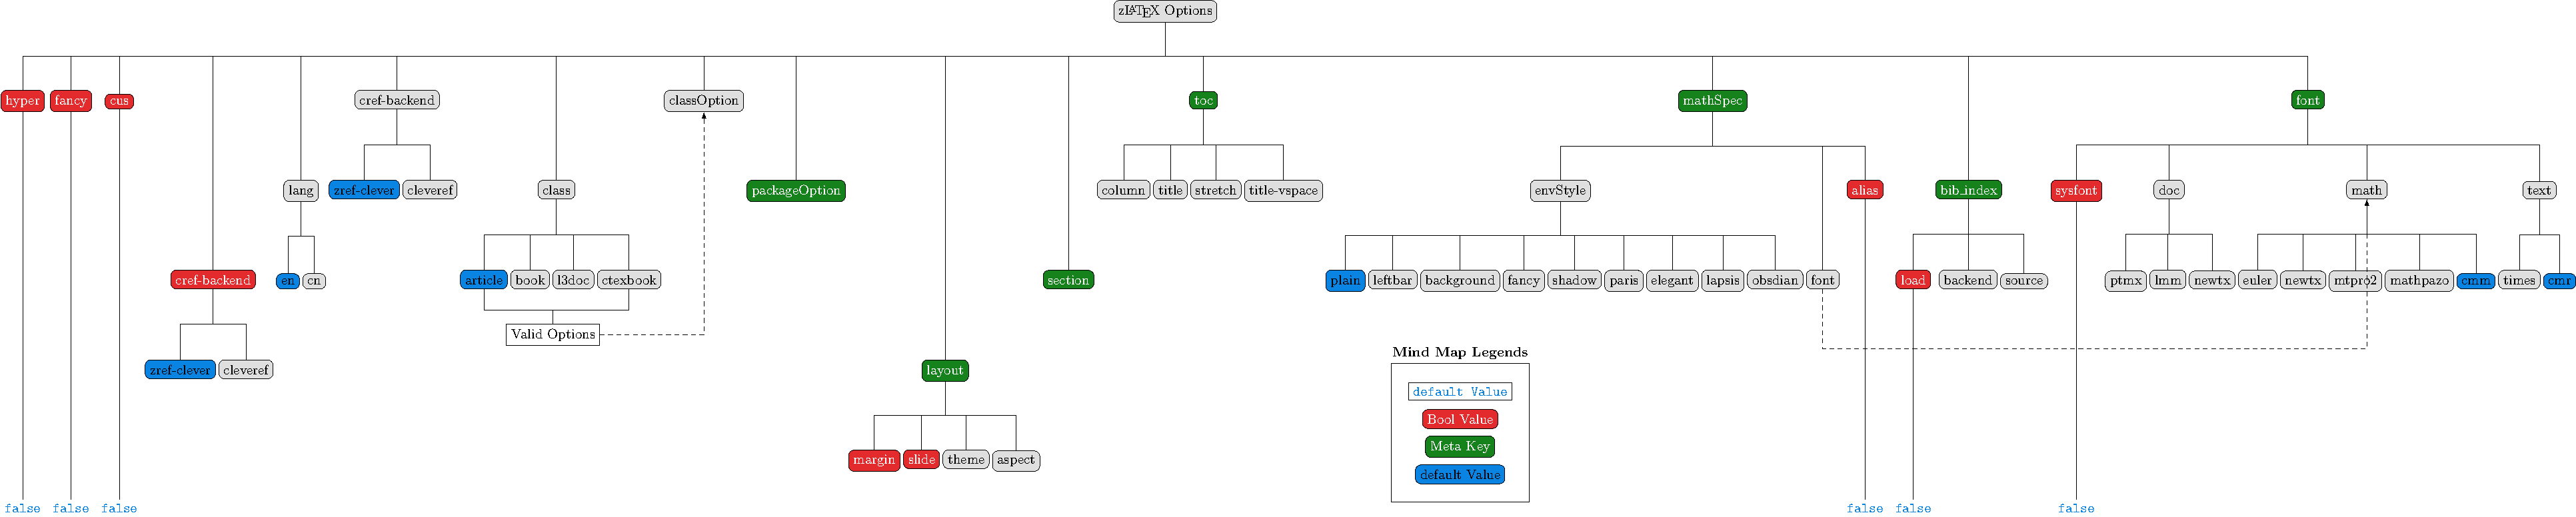
\includegraphics[width=1\linewidth]{ztex_options.pdf}
  \caption{\ztex{} Document Class Options Diagram}
  \label{fig:ztex-options}
\end{figure}

Overall, the document class options of \ztex{} are relatively complex. For users new to this document class, it's not necessary to know all configuration options, as \ztex{} already produces good results with default settings. Below, we will detail the specification methods and meanings of each \meta{key}.

\begin{function}[updated=2025-04-25]{\ztexloadmod, \ztexloadlib}
  \begin{syntax}
    \cs{ztexloadmod}\marg{module name}
    \cs{ztexloadlib}\marg{library name}
  \end{syntax}
  These commands can be used to load modules and libraries of \ztex{}. All modules are loaded by default, while libraries are not loaded by default and need to be specified by users. The current lists of modules and libraries are as follows:

  \noindent\parbox[t]{.5\linewidth}{
    \noindent \textbf{Module List:}
    \begin{itemize}
      \item \file{ztex.module.font.tex}
      \item \file{ztex.module.ref.tex}
      \item \file{ztex.module.page.tex}
      \item \file{ztex.module.color.tex}
      \item \file{ztex.module.thm.tex}
      \item \file{ztex.module.sect.tex}
    \end{itemize}}%
  \parbox[t]{.5\linewidth}{
    \noindent \textbf{Library List:}
    \begin{itemize}
      \item \file{ztex.library.fancy.tex}
      \item \file{ztex.library.alias.tex}
      \item \file{ztex.library.slide.tex}
      \item \file{ztex.library.thm.tex}
    \end{itemize}}
\end{function}

The loading methods for each module and library are shown in the following example:
\begin{DocExample}
% \documentclass{ztex}
\ztexloadlib/\zarg{fancy}/
\ztexloadlib/\zarg{alias}/
\ztexloadlib/\zarg{slide}/
\ztexloadlib/\zarg{thm}/
\end{DocExample}

You can certainly write your own module, let's assume its name is \meta{moduleA}. Name this file \texttt{ztex.module.\meta{moduleA}.tex}, place it under the path \meta{z\TeX}\file{/module/}, and then load it with the following command:
\begin{DocExample}
\ztexloadmod{/\meta{moduleA}/}
\end{DocExample}

\begin{function}[rEXP, updated=2024-11-05]{lang}
  \begin{syntax}
    lang=\meta{cn, \zdefault*{en}}
  \end{syntax}
  Currently, \ztex{} only supports Chinese and English, with partial support for French. Depending on the document class language, \ztex{} loads different language-related packages\index{language packages}. The package loading under different \meta{lang} settings is as follows:
\end{function}
\begin{table}[!htb]
  \begin{tblr}{
    colspec={|X[1, c]|X[1.5, c]|X[1, c]|X[1, c]|X[1, c]|},
    rowspec={|Q[m]|Q[m]|}
  }
  lang=en & \pkg{inputenc}(\hologo{pdfTeX}) & \pkg{fontenc} & \pkg{babel} & \pkg{microtype} \\
  lang=cn & \pkg{fontspec} & \pkg{ctex} \\
  \end{tblr}
  \caption{\ztex{} Document Class Language Packages}
  \label{tab:lang-package}
\end{table}

\begin{function}[rEXP, updated=2024-11-05]{hyper}
  \begin{syntax}
    hyper=\meta{true, \zdefault*{false}} 
  \end{syntax}
  Whether to enable internal document hyperlinks and PDF bookmarks. Default is \ztexverb{false}. It is recommended to enable this option in the final draft, while setting it to \ztexverb{false} during the drafting stage can speed up compilation.
\end{function}

\begin{function}[rEXP, updated=2024-11-05]{fancy}
  \begin{syntax}
    fancy=\meta{true, \zdefault*{false}} 
  \end{syntax}
  This option controls the document's appearance, including section styles and theorem-like environment styles. Default is \ztexverb{false}. 
\end{function}

\begin{function}[rEXP, updated=2024-11-05]{class}
  \begin{syntax}
    class=\meta{\zdefault*{article}, book, ctexbook} 
  \end{syntax}
  This option specifies the base document class to load. Default is \cls{article}. After loading the \cls{ctexbook} document class, you can use its \cmd{\ctexset} command for configuration.
\end{function}

\begin{function}[rEXP, updated=2024-11-05]{classOption}
  \begin{syntax}
    classOption=\meta{class options} 
  \end{syntax}
  This option accepts a comma-separated list to pass base document class options. For the default \cls{article} document class, this is \ztexverb{oneside, 12pt}. A simple configuration example:
\begin{DocExample}
\documentclass[
  class=article,
  classOption={10pt, leqno, a4paper},
]{ztex}
\end{DocExample}
\end{function}

\begin{function}[rEXP, updated=2024-11-20]{packageOption}
  \begin{syntax}
    packageOption=\meta{key-value} 
  \end{syntax}
  This option accepts key-value pairs to pass options to different packages. Example usage:
\end{function}
\begin{DocExample}
\documentclass[
  packageOption={
    fontspec=quiet, 
    ctex={scheme=plain, punct=quanjiao},
  },
]{ztex}
\end{DocExample} 

\begin{function}[updated=2024-12-25]{toc}
  \begin{syntax}
    toc=\meta{key-value}
  \end{syntax}
  This option sets the table of contents style. All available configurations are:
\end{function}
\begin{DocExample}
\ztexset{
  toc={
    column=/\meta{int\zdefault{1}}/,
    title=/\meta{tl\zdefault{Contents}}/,
    title-vspace=/\meta{dim\zdefault{-2em}}/,
    stretch=/\meta{float\zdefault{1}}/
  }
}
\end{DocExample}
If the above $\meta{column} \ge 2$, \ztex{} will automatically load the \pkg{multicol} package. Note: Since document class options in \LaTeX{} cannot contain control sequences, if any sub-item of \meta{toc} contains control sequences, it must be set through the command \cmd{\ztexset}. Example:
\begin{DocExample}
\ztexset{
  toc={
      title=\hfill\large\normalfont CONTENTS {\sffamily\small NEW}\hfill
    }
}
\end{DocExample}

\begin{function}[rEXP, updated=2024-12-06]{font}
  \begin{syntax}
    font = \meta{key-value}
  \end{syntax}
  This option is currently experimental and mainly for font configuration. Default is \ztexverb{false}. When enabled, \ztex{} will automatically load the \pkg{fontspec} package, requiring the engine to be switched to \hologo{XeLaTeX} or \hologo{LuaLaTeX}. Current available options:
\end{function}
\begin{DocExample}
\documentclass[
  font={config=/\meta{true, \zdefault*{false}}/}
]{ztex}
\end{DocExample}

\begin{function}[rEXP, updated=2024-11-05]{layout}
  \begin{syntax}
    layout=\meta{key-value}
  \end{syntax}
  Set document layout. All available configurations:
\end{function}
\begin{DocExample}
\documentclass[
  layout={
    margin=/\meta{bool\zdefault{false}}/,
    slide=/\meta{bool\zdefault{false}}/,
    aspect=/\meta{float|float\zdefault{12|9}}/,
    theme=/\meta{str\zdefault{AnnArborDefault}}/
  },
]{ztex}
\end{DocExample}
After loading the \file{slide} library, if \meta{slide}\texttt{=true} is set, the document can be switched to slide mode.

\begin{function}[updated=2024-12-05]{bib_index}
  \begin{syntax}
    bib_index=\meta{key-value}
  \end{syntax}
  This option controls whether the document generates indexes and references. All available options:
\end{function}
\begin{DocExample}
\ztexset{
  bib_index={
    load=/\meta{bool\zdefault{false}}/,
    source=/\meta{str\zdefault{ref.bib}}/,
    backend=/\meta{str\zdefault{biber}}/
  }
}
\end{DocExample}
\meta{load} controls whether to load the \pkg{biblatex} package. Default is \ztexverb{false}. \meta{source} specifies the reference source file, defaulting to \file{ref.bib}. \meta{backend} specifies the reference backend, defaulting to {biber}.

\begin{function}[updated=2024-11-05]{mathSpec}
  \begin{syntax}
    mathSpec=\meta{key-value}
  \end{syntax}
  This key configures math typesetting options. All available options:
\end{function}
\begin{DocExample}
\ztexset{
  mathSpec={
    alias=/\meta{bool\zdefault{false}}/,
    envStyle=/\meta{tl\zdefault{plain}}/,
    font=/\meta{choice\zdefault{ncmrm}}/
  }
}
\end{DocExample}

\meta{alias} defaults to \ztexverb{false}. When set to \ztexverb{true}, \ztex{} loads the \file{alias} library, which contains shorthand declarations for a series of commands, such as \cmd{\ZZ} for \ztexverb{\mathbb{Z}}. \meta{envStyle} specifies the style of math environments, defaulting to \ztexverb{plain}. For compilation speed considerations, although \ztex{} predefines a series of environment styles, it does not preload all styles, instead moving some to the \file{theme} library. The detailed predefined style list is:

\noindent\parbox[t]{.5\linewidth}{
\noindent \textbf{\pkg{thm} module defined styles}:
\begin{itemize}
  \item plain 
  \item background
  \item leftbar 
  \item fancy 
\end{itemize}}%
\parbox[t]{.5\linewidth}{
\noindent \textbf{\pkg{theme} library defined styles}:
\begin{itemize}
  \item shadow
  \item paris 
  \item elegant
  \item obsidian
  \item lapsis
\end{itemize}}

\meta{font} specifies the math formula font. Predefined fonts include: \texttt{newtx, euler, mtpro2, mathpazo, ptmx}. Among these, \ztexverb{mtpro2} is a paid font and requires manual installation by users.

% ----------------------------------------------------------------------
%                              Implement
% ----------------------------------------------------------------------
% \cleardoublepage
% \newgeometry{left=1in, top=.75in, right=.9in, bottom=.75in}
% \ztexslideTF{}{
%   \section{\ztex{} Implementation}
%   \pagestyle{empty}
%   \zpagemask*[anchor=mr, position={(\zpw, .5\zph)}]{{\sffamily\color{gray}\scalebox{5}{\thepage}}}
%   \renewcommand{\theFancyVerbLine}{\sffamily
%     \textcolor{gray}{\small\oldstylenums{\arabic{FancyVerbLine}}}}
%   \setminted{ bgcolor=, linenos=true, numbers=both }


%   \subsection{ztex.cls}
%   \inputminted{latex}{../code/ztex.cls}

%   \newpage
%   \subsection{module.font}
%   \inputminted{latex}{../code/module/ztex.module.font.tex}

%   \newpage
%   \subsection{module.ref}
%   \inputminted{latex}{../code/module/ztex.module.ref.tex}

%   \newpage
%   \subsection{module.page}
%   \inputminted{latex}{../code/module/ztex.module.page.tex}

%   \newpage
%   \subsection{module.color}
%   \inputminted{latex}{../code/module/ztex.module.color.tex}

%   \newpage
%   \subsection{module.thm}
%   \inputminted{latex}{../code/module/ztex.module.thm.tex}

%   \newpage
%   \subsection{module.sect}
%   \inputminted{latex}{../code/module/ztex.module.sect.tex}

%   \newpage
%   \subsection{library.fancy}
%   \inputminted{latex}{../code/library/ztex.library.fancy.tex}

%   \newpage
%   \subsection{library.alias}
%   \inputminted{latex}{../code/library/ztex.library.alias.tex}

%   \newpage
%   \subsection{library.slide}
%   \inputminted{latex}{../code/library/ztex.library.slide.tex}

%   \newpage
%   \subsection{library.thm}
%   \inputminted{latex}{../code/library/ztex.library.thm.tex}
% }


% \clearpage
% \PrintIndex
\end{document}